\section{Simulation Initializations}
\label{apdx:simulation-initializations}

\subsection{Exogenous variables}
The law of motion for labor is given by:

\begin{equation}
    N_{t+1} = N_t \left(\frac{N_\infty}{N_t}\right)^{\delta^N}
\end{equation}

\begin{table}[ht]
\centering
\begin{tabular}{lccc}
    \toprule
    Parameter & Symbol & Value DICE 2016 & Value DICE 2023 \\
    \midrule
    World pop. (Millions) & \(N_0\) & 7403 & 7752.9 \\
    Asymptotic world pop (Millions) & \(N_\infty\) & 11500 & 10825.0 \\
    Convergence rate & \(\delta^N\) & 0.134 & 0.145 \\
    \bottomrule
\end{tabular}
\caption{Labor Evolution Parameterization}
\label{table:labor_parameters}
\end{table}

\begin{figure}[h]
    \centering
    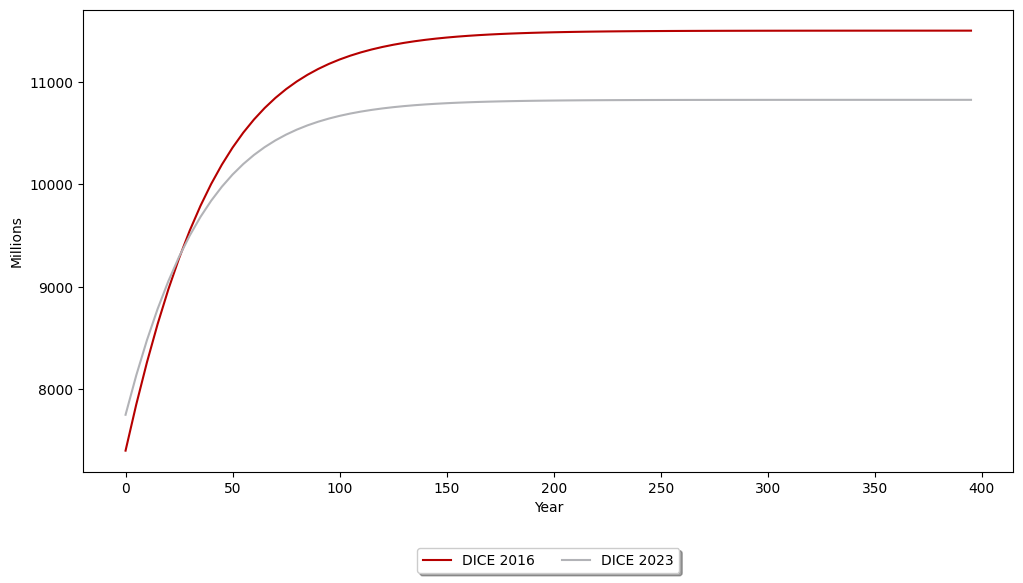
\includegraphics[width=1.0\textwidth]{images/appendix/initial values/labor.png}
    \caption{Exogenous law of motion for labor}
    \label{fig:labor_law_of_motion}
\end{figure}


Total factor productivity evolves according to:

\begin{equation}
    A_{t+1} = \frac{A_t}{1-g_t^A}, \quad \text{with}
\end{equation}

\begin{equation}
    g_{t+1}^A = g_0^A \exp\left(-\delta^A \Delta (t-1)\right)
\end{equation}


\begin{table}[ht]
\centering
\begin{tabular}{lccc}
    \toprule
    Parameter & Symbol & Value DICE 2016 & Value DICE 2023 \\
    \midrule
    Initial TFP & \(A_0\) & 5.115 & 5.84 \\
    Initial TFP Growth (pr. 5yrs) & \(g_0^A\) & 0.075 & 0.066 \\
    Decline Rate of TFP Growth & \(\delta^A\) & 0.005 & 0.015 \\
    Time Step & \(\Delta\) & 5 & 5 \\
    \bottomrule
\end{tabular}
\caption{TFP Evolution Parameterization}
\label{table:tfp_parameters}
\end{table}

\begin{figure}[h]
    \centering
    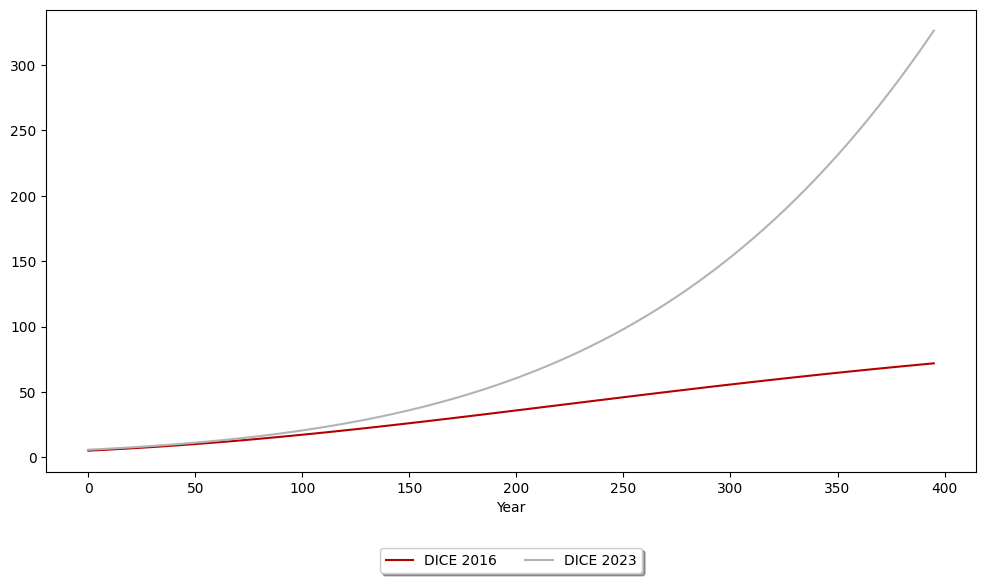
\includegraphics[width=1.0\textwidth]{images/appendix/initial values/tfp.png}
    \caption{Exogenous law of motion for tfp}
    \label{fig:tfp_law_of_motion}
\end{figure}


Carbon intensity relates anthropogenic carbon emissions to economic production and is a fraction of total output. DICE 2016 uses:

\begin{equation}
    \sigma_{t+1} = \exp(g_t^\sigma \Delta)
\end{equation}

\begin{equation}
    g_{t+1}^\sigma = g_t^\sigma \left( 1 + \delta^\sigma \right)^\Delta
\end{equation}



While DICE 2023 uses:

\begin{equation}
    \sigma_{t+1} = \sigma_t \exp \left( \Delta g_t^\sigma \right) \mathfrak{e}_{t+1}
\end{equation}

\begin{equation}
    g_{t}^\sigma = \min (g_0^\sigma (\delta^\sigma)^{t-1}, g_\infty^\sigma) 
\end{equation}

The current ratio of \(\text{CO}_2\)e to industrial \(\text{CO}_2\) is:
\begin{equation}
    \mathfrak{e}_t = \begin{cases}
        \mathfrak{e}_{2020} + \frac{\mathfrak{e}_{2100} - \mathfrak{e}_{2020}}{16} (t - 1), & \text{if } t \leq 16 \\
        \mathfrak{e}_{2100} - \mathfrak{e}_{2020}, & \text{if } t \geq 17
    \end{cases}
\end{equation}


And both using:
\begin{equation}
    \sigma_0 = \frac{E_0}{Y_0 (1-\mu_0)}
\end{equation}

\begin{table}[ht]
\centering
\begin{tabular}{lccc}
    \toprule
    Parameter & Symbol & Value DICE 2016 & Value DICE 2023 \\
    \midrule
    Initial growth of sigma (pr. yr.) & \(g_0^\sigma\) & -0.0152 & -0.015 \\
    Decline rate of decarbonization & \(\delta^\sigma\) & -0.001 & 0.96 \\
    Initial Industrial Emissions (GtCO$_2$) & \(E_0\) & 35.85 & 37.56 \\
    Initial World Gross Output (trillion\$) & \(Y_0\) & 105.5 & 135.7 \\
    Initial Abatement Rate & \(\mu_0\) & 0.03 & 0.05 \\
    Time Step & \(\Delta\) & 5 & 5 \\
    Ratio of CO$_2$e to industrial CO$_2$ 2020 & \(\mathfrak{e}_{2020}\) & - & 1.40 \\
    Ratio of CO$_2$e to industrial CO$_2$ 2100 & \(\mathfrak{e}_{2100}\) & - & 1.21 \\
    \bottomrule
\end{tabular}
\caption{Carbon Intensity Evolution Parameterization}
\label{table:carbon_intensity_parameters}
\end{table}

\begin{figure}[h]
    \centering
    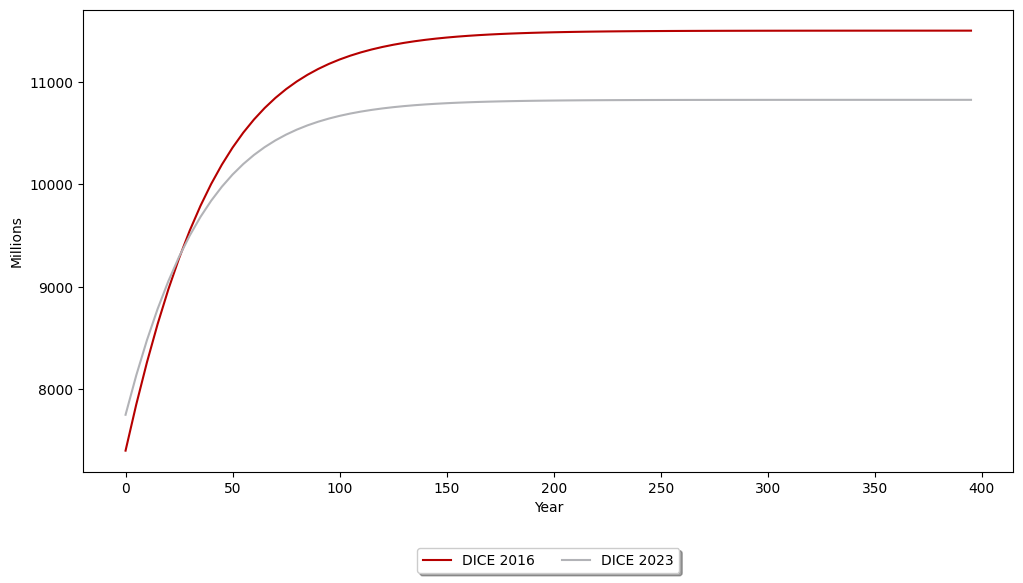
\includegraphics[width=1.0\textwidth]{images/appendix/initial values/labor.png}
    \caption{Exogenous law of motion for carbon intensity}
    \label{fig:carbon_intensity_law_of_motion}
\end{figure}



Abatement costs depend on this backstop price that is calculated differently between the two model versions. The 2016 version is given as:

\begin{equation}
    p_t^{\text{back}} = \tilde p (1-g^\text{back})^{t-1 }
\end{equation}

The 2023 version is as follows: 

\begin{equation}
    p_t^{\text{back}} = 
    \begin{cases} 
       \bar p \times \exp(-\Delta \times 0.01 \times (t - 7)), & \text{if } t \leq 7 \\
       \bar p \times \exp(-\Delta \times 0.001 \times (t - 7)), & \text{if } t > 7 
    \end{cases}
\end{equation}

Abatement costs in both versions are given by:

\begin{equation}
    \theta_{1,t} = \frac{p_t^{\text{back}} \sigma_t}{1000\theta_2}
\end{equation}

\begin{table}[ht]
\centering
\begin{tabular}{lccc}
    \toprule
    Parameter & Symbol & Value DICE 2016 & Value DICE 2023 \\
    \midrule
    Initial growth of sigma (pr. yr.) & \(g_0^\sigma\) & -0.0152 & -0.015 \\
    Decline rate of decarbonization & \(\delta^\sigma\) & -0.001 & 0.96 \\
    Initial Industrial Emissions (GtCO$_2$) & \(E_0\) & 35.85 & 37.56 \\
    Initial World Gross Output (trillion\$) & \(Y_0\) & 105.5 & 135.7 \\
    Initial Abatement Rate & \(\mu_0\) & 0.03 & 0.05 \\
    Time Step & \(\Delta\) & 5 & 5 \\
    Ratio of CO$_2$e to industrial CO$_2$ 2020 & \(\mathfrak{e}_{2020}\) & - & 1.40 \\
    Ratio of CO$_2$e to industrial CO$_2$ 2100 & \(\mathfrak{e}_{2100}\) & - & 1.21 \\
    \bottomrule
\end{tabular}
\caption{Abatement Cost Evolution Parameterization}
\label{table:abatement_cost_parameters}
\end{table}

Emissions from deforestation in the 2016 version are given by:

\begin{equation}
    E_t^\text{land} = E_0^\text{land}(1-\delta^\text{land})^{t-1}
\end{equation}


\begin{table}[ht]
\centering
\begin{tabular}{lccc}
    \toprule
    Parameter & Symbol & Value DICE 2016 & Value DICE 2023 \\
    \midrule
    Initial Land Use Emissions & \(E_0^\text{land}\) & 2.6 & 5.9 \\
    Land Use Decline Rate (yr.) & \(\delta^{\text{forest}}\) & 0.115 & 0.1 \\
    \bottomrule
\end{tabular}
\caption{Land Use Emissions Evolution Parameterization}
\label{table:emissions_parameters}
\end{table}

\begin{figure}[H]
    \centering
    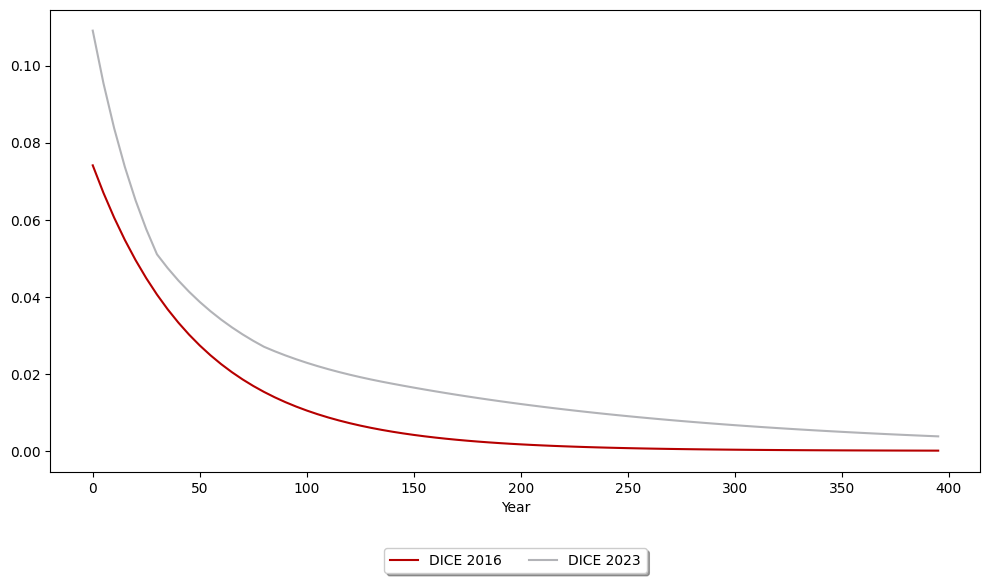
\includegraphics[width=1.0\textwidth]{images/appendix/initial values/abatement costs.png}
    \caption{Exogenous law of motion for abatement costs}
    \label{fig:abatement_costs_law_of_motion}
\end{figure}


\subsection{Endogenous Variables}

\textbf{Economic parameterization.} The discount rate is initialized as:
\begin{equation}
    \beta = \left( \frac{1}{1+\rho} \right)^\Delta
\end{equation}

\begin{table}[H]
\centering
\begin{tabular}{l|lll}
    \toprule
    Calibrated Parameter & Symbol & Value & Model \\
    \midrule
    Pure Rate of Time Preference & \(\rho\) & 0.0286 & ACE \\
    Capital Share of Output & \(\kappa\) & 0.3 & ACE \\
    Capital Depreciation Factor & \(\delta_k\) & 0.0439 & ACE \\
    Growth Rate of Capital & \(g_k\) & 0.02949 & ACE \\
    Time Step & \(\Delta\) & 5 & DICE (All) \\
    Initial Capital Stock 2015 (trillion 2010\$) & \(K_0\) & 223 & DICE 2016 \\
    Initial Capital Stock 2020 (trillion 2019\$) & \(K_0\) & 295 & DICE 2023 \\
    Damage parameter & \(\xi_0\) & 0.02219 & ACE \\
    Parameter & \(\xi_1\) & \(\frac{\log 2}{s}=0.2310, \;s=3\) & ACE \\
    \bottomrule
\end{tabular}
\caption{Generic Parameterization of the Economy}
\label{table:economic_parameters}
\end{table}


\textbf{Carbon parameterization.} The vector that initializes DICE's 5-year step carbon cycle's transition matrix is given in \textcite{TraegerChristian2023ACE} and is

\begin{equation}
    \Xi = \begin{bmatrix}
        0.088 & 0.0025 & 0.03832888889 & 0.00033750
    \end{bmatrix}
\end{equation}

The components of the transition matrix are constructed as:
\begin{equation}
    \Phi = 
    \begin{bmatrix}
        1 - \Xi_1 & \Xi_3       & 0 \\
        \Xi_1     & 1 - \Xi_2   & \Xi_4 \\
        0         & \Xi_2       & 1 - \Xi_4
    \end{bmatrix}
\end{equation}


\begin{table}[ht]
\centering
\begin{tabular}{lcc}
    \toprule
    Parameter & Symbol & ACE \\
    \midrule
    Atmospheric Carbon Stock 2015 (GtC) & \(M_{1,0}\) & 862.86 \\
    Upper Ocean Carbon Stock 2015 (GtC) & \(M_{2,0}\) & 1541.11 \\
    Deep Ocean Carbon Stock 2015 (GtC) & \(M_{3,0}\) & 10010.44 \\
    \bottomrule
\end{tabular}
\caption{Generic Parameterization of the Carbon Reservoirs}
\label{table:carbon_stock_parameters}
\end{table}


\textbf{Temperature parameterization.}

\begin{table}[ht]
\centering
\begin{tabular}{lcc}
    \toprule
    Parameter & Symbol & Value ACE \\
    \midrule
    Temperature Layer 1 & \(\tau_{1,0}\) & $\sim 1.2567272$ \\
    Temperature Layer 2 & \(\tau_{2,0}\) & $\sim 1.1854651$ \\
    Heat to space & \(\sigma^\text{up}_1\) & $0.24755$ \\
    Heat from second to first layer & \(\sigma^\text{up}_2\) & $0.011354$ \\
    Heat from first to second layer & \(\sigma^\text{down}_1\) & $0.1479$ \\
    \bottomrule
\end{tabular}
\caption{Generic Parameterization of Temperatures}
\label{table:temperature_parameters}
\end{table}

The transition matrix for the two-layer temperature model is given by:
\begin{equation}
    \begin{bmatrix}
        1-\sigma^\text{up}_1-\sigma^\text{down}_1 & \sigma^\text{down}_1 \\
        \sigma^\text{up}_2 & 1 - \sigma^\text{up}_2
    \end{bmatrix}
\end{equation}

Furthermore, \(\sigma^\text{forc}\) is given by:
\begin{equation}
    \sigma^\text{forc} = 1-\bm{\sigma}_{1,1} - \bm{\sigma}_{1,2}
\end{equation}